\documentclass[border=8pt]{standalone}
\usepackage{tikz}
\usetikzlibrary{arrows.meta,positioning,fit,calc}
\definecolor{cjob}{RGB}{72,116,158}
\definecolor{cmac}{RGB}{86,156,104}
\definecolor{cpm}{RGB}{198,86,76}
\definecolor{cgray}{RGB}{245,245,245}
\begin{document}
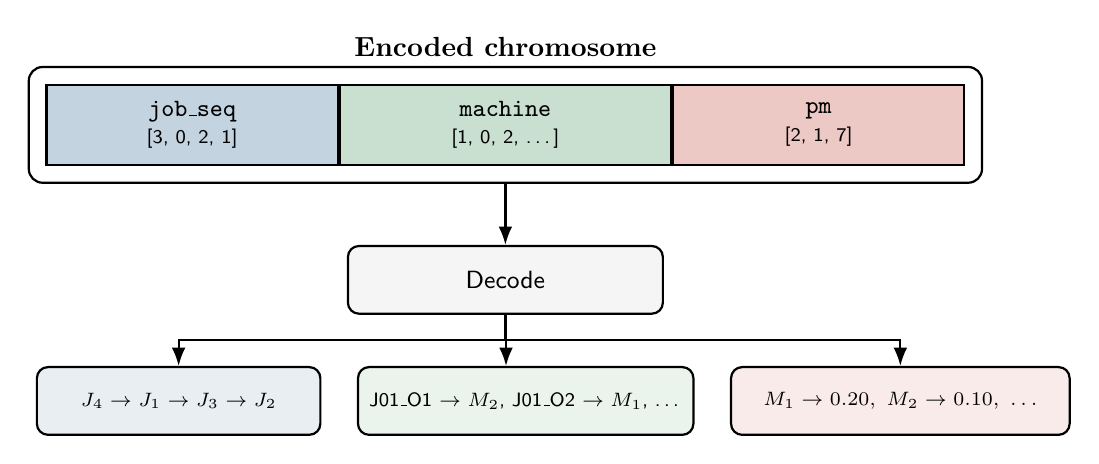
\begin{tikzpicture}[
  font=\sffamily\small,
  >=Latex,
  part/.style={draw,thick,minimum height=1.02cm,align=center,inner xsep=2.5mm},
  box/.style={draw,thick,rounded corners=4pt,minimum height=0.86cm,align=center,inner sep=4pt},
  arrow/.style={->,thick}
]
  \node[part,fill=cjob!32,minimum width=3.7cm] (job)
    {\texttt{job\_seq}\\[-1pt]\scriptsize [3, 0, 2, 1]};
  \node[part,fill=cmac!32,minimum width=4.2cm,right=0pt of job] (mac)
    {\texttt{machine}\\[-1pt]\scriptsize [1, 0, 2, \ldots]};
  \node[part,fill=cpm!32,minimum width=3.7cm,right=0pt of mac] (pm)
    {\texttt{pm}\\[-1pt]\scriptsize [2, 1, 7]};
  \node[draw,thick,rounded corners=5pt,fit=(job)(mac)(pm),inner sep=6pt,
        label={[font=\bfseries]above:Encoded chromosome}] (chrom) {};

  \node[box,fill=cgray,below=1.0cm of mac,minimum width=4.0cm] (decode)
    {Decode};
  \node[box,fill=cjob!12,below=0.65cm of decode,xshift=-4.15cm,minimum width=3.6cm] (jobout)
    {\scriptsize $J_4 \rightarrow J_1 \rightarrow J_3 \rightarrow J_2$};
  \node[box,fill=cmac!12,right=0.45cm of jobout,minimum width=4.1cm] (macout)
    {\scriptsize J01\_O1 $\rightarrow M_2$, J01\_O2 $\rightarrow M_1$, \ldots};
  \node[box,fill=cpm!12,right=0.45cm of macout,minimum width=4.3cm] (pmout)
    {\scriptsize $M_1 \rightarrow 0.20,\ M_2 \rightarrow 0.10,\ \ldots$};

  \coordinate (split) at ($(decode.south)+(0,-0.32)$);
  \draw[arrow] (chrom.south) -- (decode.north);
  \draw[thick] (decode.south) -- (split);
  \draw[arrow] (split) -| (jobout.north);
    \draw[arrow] (split) -| ($(macout.north)-(0.25cm,0)$);
  \draw[arrow] (split) -| (pmout.north);
\end{tikzpicture}
\end{document}
